\documentclass{article}
\usepackage[utf8]{inputenc}
\usepackage{amssymb}
\usepackage{graphicx}
\usepackage[pdftex]{pict2e}
\usepackage[dvipsnames]{xcolor}
\setlength{\unitlength}{1cm}
\setlength{\fboxsep}{4pt}
\usepackage{hyperref}
\usepackage{subfig}
\usepackage{tikz} \graphicspath { {./images/} }


\begin{document}

\textbf{ The idea of drawing graphs on a 2d plane might not be a vague idea to the readers.  Since middle school we've encountered 
    plots like y=x y = squared of x on the board of our maths class. Still can't picture it here are a few of them drawn below hope it 
creates a deja vu in your mind .}


\begin{center}
    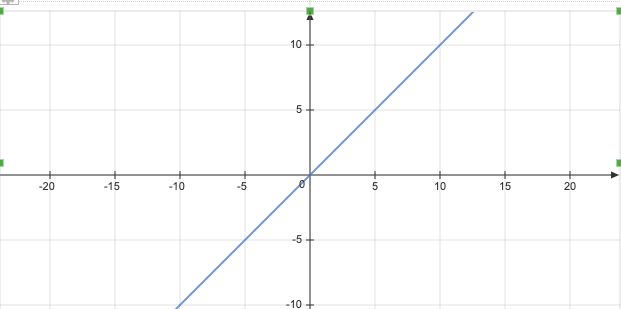
\includegraphics[scale = 7.0,width =7cm] {images/Screen Shot 2022-05-28 at 18.38.15.png}
\end{center}

\begin{center}
    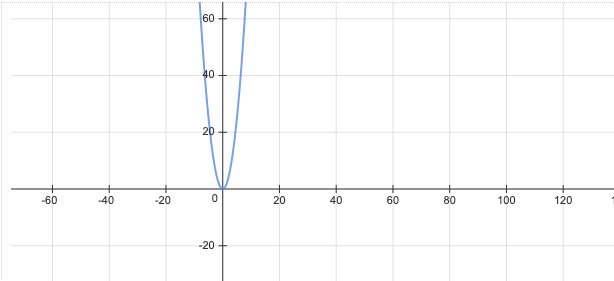
\includegraphics[scale = 7.0, width =7cm] {images/Screen Shot 2022-05-28 at 18.39.24.png}
\end{center}

\begin{center}
    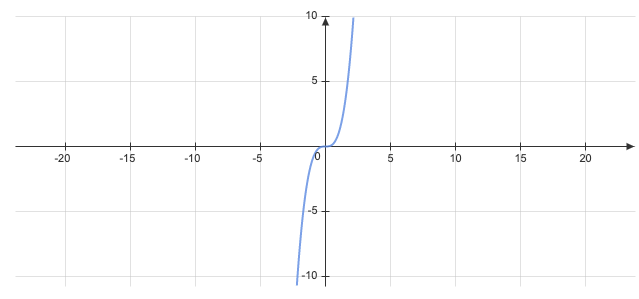
\includegraphics[scale = 7.0, width=7cm] {images/Screen Shot 2022-05-28 at 18.50.37.png}
\end{center}

\textbf{The first plot represents the line y = x , The second plot represents the curve \[ y = (x ^ {2}) \] and the third plot represents the curve
\[ y = ( x ^{3} ) \] }


\end{document}

